\chapter{Introduzione}
\label{ch:introduzione}

In questo capitolo introduttivo si intende descrivere il contesto e le
motivazioni che hanno portato allo sviluppo di questo elaborato. Si presenta una
panoramica generale del campo di studio in cui l'argomento si colloca, ma non
solo: sebbene il lavoro si sia concentrato su un'implementazione reale, si
vogliono presentare anche l'importanza e i benefici che tali tecnologie possono
portare ad altri algoritmi e applicazioni, ponendo particolare attenzione ai vantaggi,
svantaggi ed eventuali problematiche che sono state riscontrate durante lo
sviluppo. Infine, si presentano gli obiettivi sperimentali che si intendono
raggiungere e la soluzione proposta al fine di soddisfarli.

\section{Contesto e motivazioni}
\label{sec:contesto}

Gli strumenti di simulazione sono dei meccanismi essenziali nella ricerca tecnologica
e scientifica in quanto il loro utilizzo permette di testare preventivamente le prestazioni
e il comportamento di sistemi estremamente complessi senza dover ricorrere a costose
e rischiose sperimentazioni reali. Anche se il loro utilizzo è molto diffuso, la
loro implementazione non è sempre banale e richiedono un'attenta progettazione e
sviluppo. Per di più, la complessità dei sistemi in esame può portare a realizzare
soluzioni non ottimali e poco efficienti, che, anche se funzionanti e matematicamente
corrette, possono richiedere tempi di esecuzione proibitivi. Questo porta a dover
ricorrere a soluzioni hardware più potenti e costose che riducono il costo-beneficio
dell'intero processo di simulazione. Qui trova spazio l'importanza della
revisione, dell'ottimizzazione e dell'efficientamento del codice, che permettono
di ridurre i tempi di esecuzione e della potenza di calcolo richiesta, permettendo
a una gamma molto più ampia di utenti di poter usufruire di tali strumenti.

\subsection{Reconfigurable Intelligent Surfaces (RISs) e Framework di
simulazione}
\label{subsec:risframework}

\begin{wrapfigure}
  {r}{.40\textwidth}
  \centering
  \def\stackalignment{l}{ 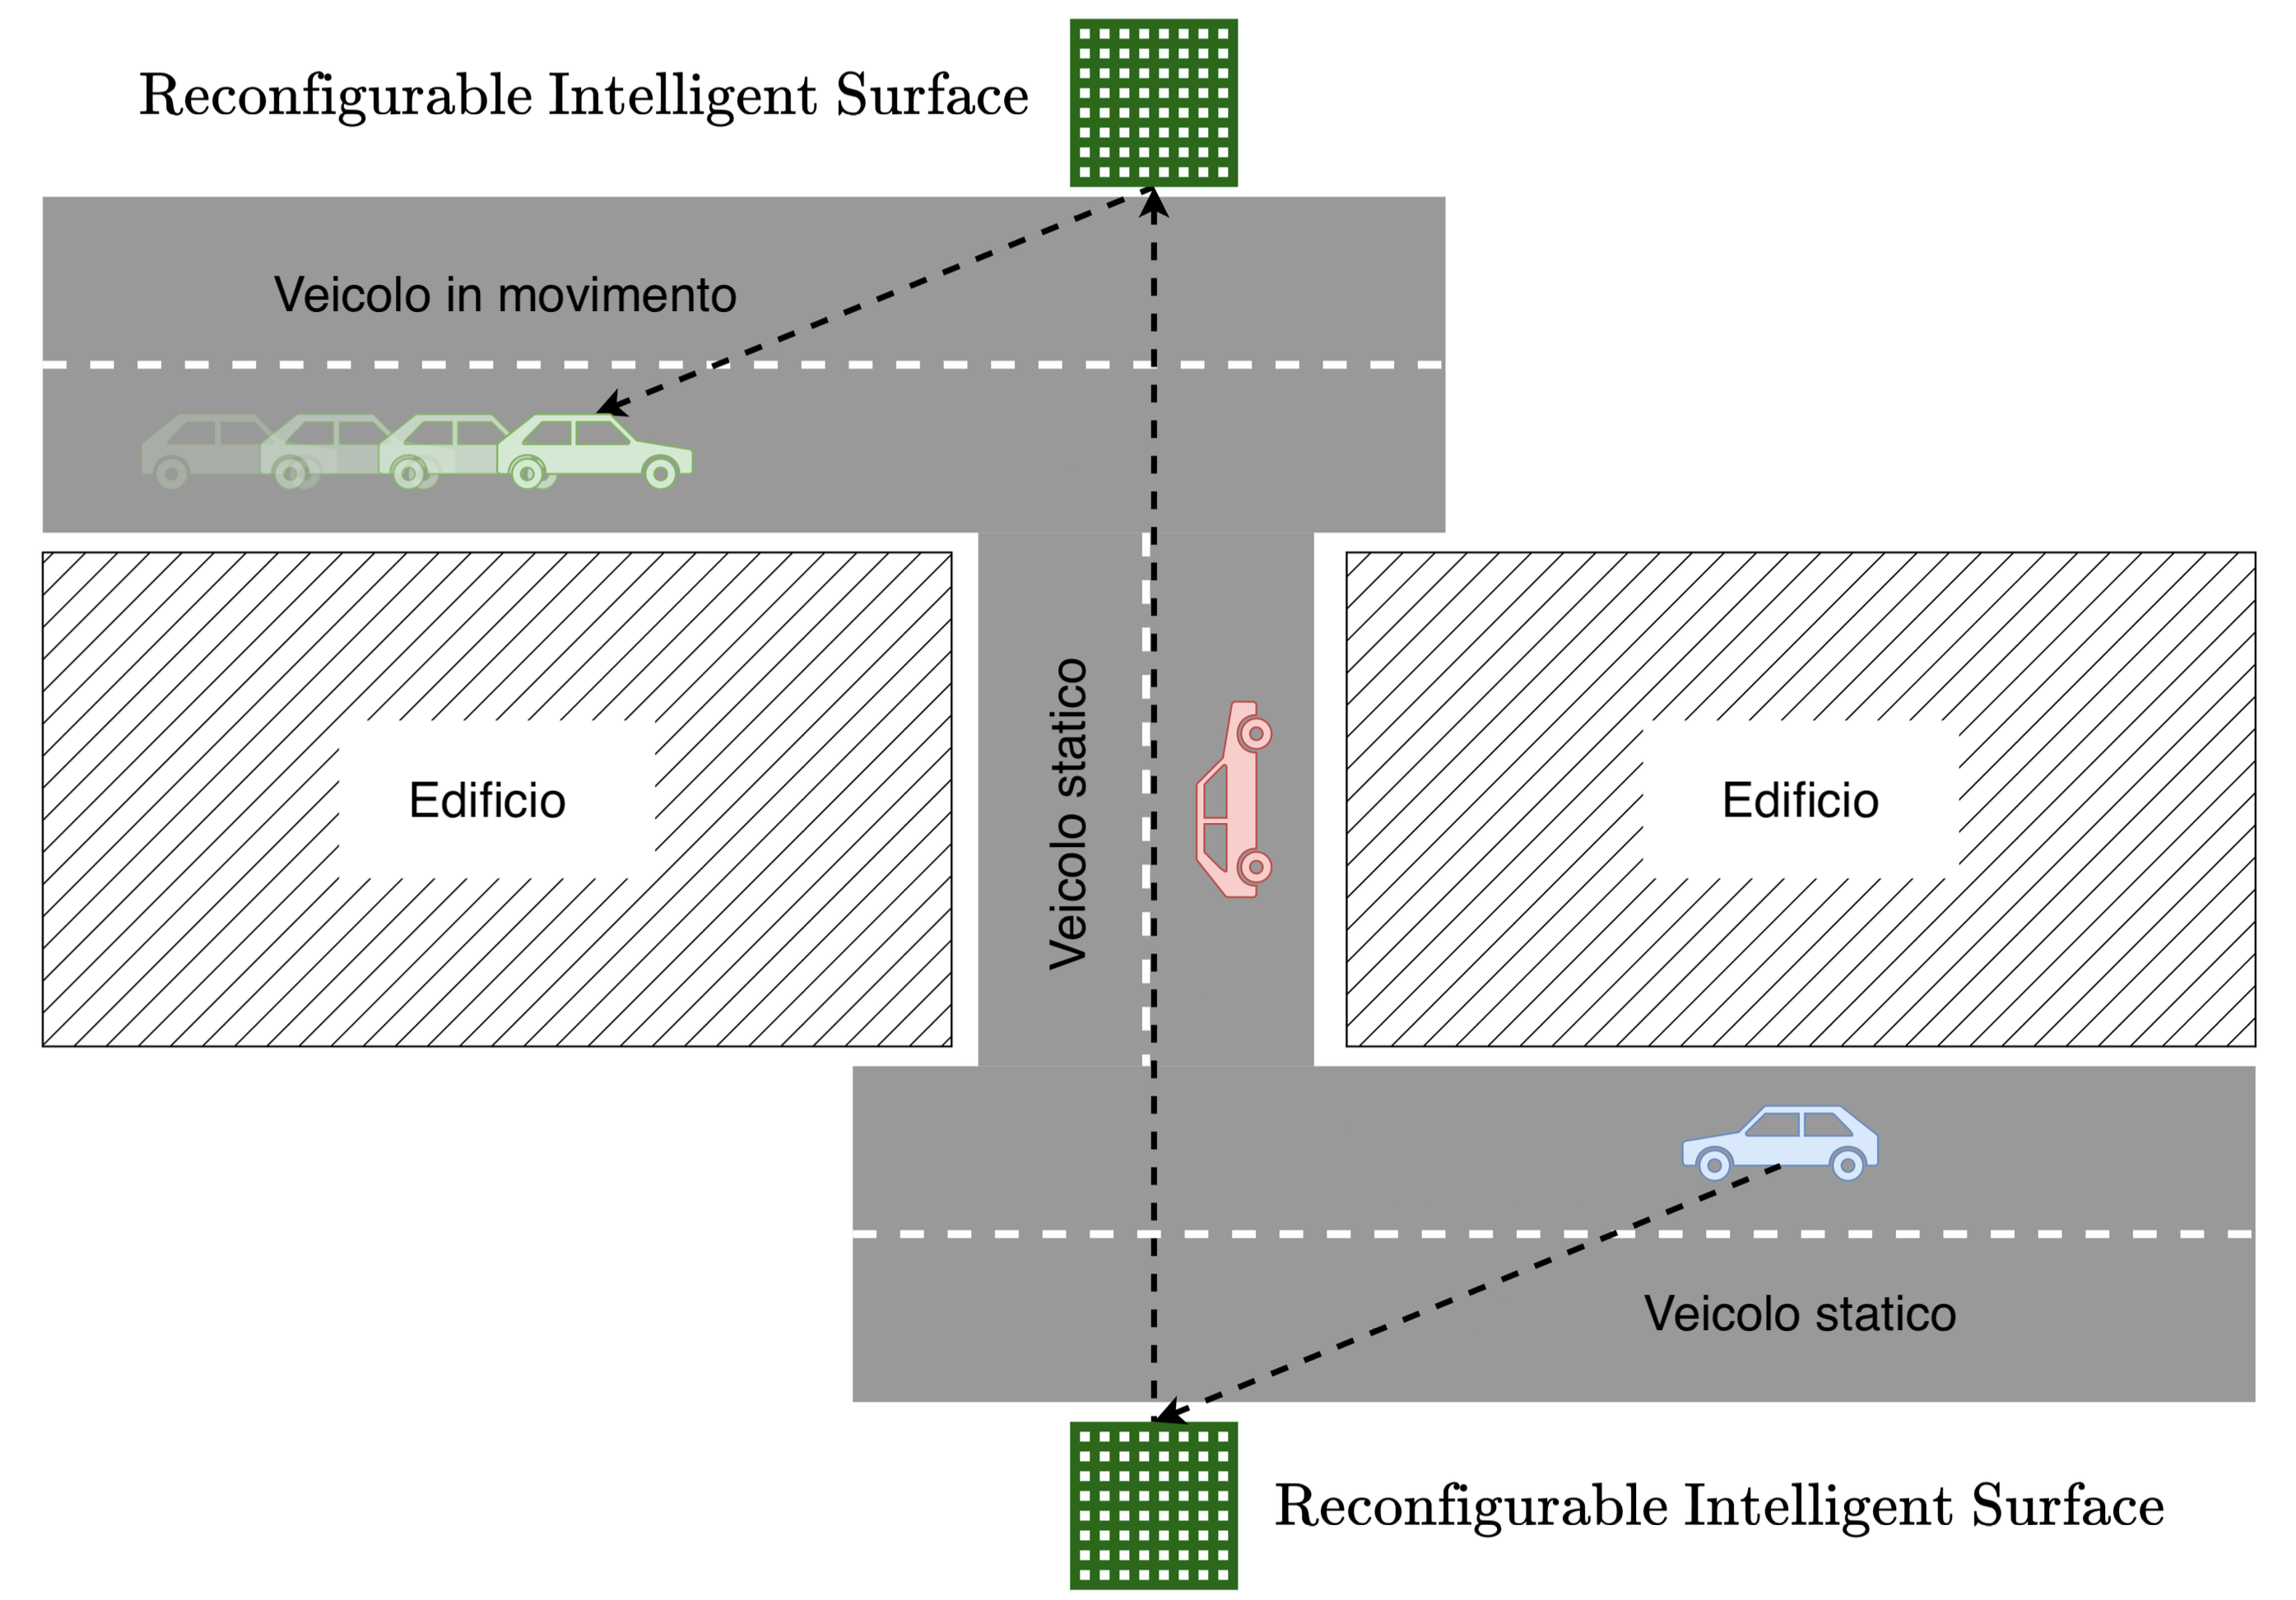
\includegraphics[width=\linewidth]{images/examples/ris-intersection.png} }
  \caption{Scenario di esempio di comunicazione tra veicoli tramite RISs\cite{cooperis}}
  \label{fig:example-ris-scenario}
  \vspace{1em}
\end{wrapfigure}

Le Reconfigurable Intelligent Surfaces (RISs) sono superfici planari programmabili
che permettono di manipolare dinamicamente le loro proprietà di riflessione in modo
da modificare la direzione in cui vengono riflesse le onde elettromagnetiche che
ci interagiscono, di fatto creando il fenomeno del \textit{beamforming}. Possono
essere sia attive, ossia amplificano il segnale riflesso, che passive, le quali si
limitano a riflettere il segnale; sono essenzialmente costituite da una griglia
di elementi radianti indipendenti, ciascuno dei quali è singolarmente ed elettronicamente
controllabile. Le RISs riscontrano molto interesse nel campo delle comunicazioni
wireless, principalmente nelle reti che sfruttano uno spettro di frequenze molto
elevato, come nelle comunicazioni che utilizzano le onde millimetriche dove la
propagazione e la penetrazione del segnale attraverso gli ostacoli e le
ostruzioni presenti nell'ambiente circostante sono molto scarse, soprattutto in situazioni
in cui non sempre è presente una diretta visibilità (LoS, Line of Sight) tra
trasmettitore e ricevitore, ad esempio in ambienti urbani o indoor. Aumenta
notevolmente la loro utilità quando si considera la loro capacità di
riconfigurazione in tempo reale, permettendo di creare canali di comunicazione dinamici
e più efficienti nei casi in cui ricevitore e trasmettitore siano in movimento,
diminuendo il rumore generato dalla naturale diffusione del segnale e
potenzialmente migliorando la comunicazione tra dispositivi terzi. Questo elaborato
è incentrato sull'ottimizzazione di una libreria sullo studio delle RISs nell'ambito
delle comunicazioni tra veicoli a guida autonoma: in particolare la libreria
\textit{CoopeRIS}\cite{cooperis} permette di simulare il comportamento di queste
superfici nell'ambito delle comunicazioni tra veicoli a guida autonoma. Di seguito
viene citato e descritto brevemente lo stack dei framework di simulazione:
\begin{itemize}
  \item \textit{SUMO} (Simulation of Urban MObility), simulatore di traffico e mobilità
    urbana\cite{sumo};

  \item \textit{OMNeT++} (Objective Modular Network Testbed), simulatore discreto
    ad eventi utilizzato maggiormente nella simulazione di reti\cite{omnetpp};

  \item \textit{Veins} (Vehicles in Network Simulation), simulatore di reti veicolari\cite{veins};

  \item \textit{PLEXE} (PLatooning EXtensions for Veins), estensione di Veins per
    la simulazione del platooning di veicoli\cite{plexe}.
\end{itemize}

\section{Contributo della Tesi}
\label{sec:contributo}

Questo elaborato si pone come obiettivo quello di migliorare la libreria in
oggetto, implementando soluzioni di ottimizzazione ed efficientamento del codice
tramite calcolo parallelo, sia mediante procedure \textit{multi-threading} che attraverso
l'utilizzo di GPU, con lo scopo finale di ridurre i tempi di esecuzione delle
simulazioni. Inoltre, assieme a queste migliorie, si propone una valutazione sia
qualitativa che quantitativa delle varie tecnologie utilizzate nei casi di studio
previsti dal paper in riferimento\cite{cooperis}, in modo da poter fornire una panoramica
completa delle migliorie ottenute, dei vantaggi e svantaggi di ciascuna
tecnologia e delle problematiche riscontrate durante lo sviluppo. La soluzione proposta
prevede di effettuare un'analisi preventiva del codice sorgente della libreria in
oggetto per identificare le eventuali criticità e i punti in cui una possibile implementazione
di calcolo parallelo potrebbe portare ai miglioramenti più significativi. In
seguito, si procederà con l'implementazione di tre soluzioni diverse,
consultabili alla tabella \ref{tab:soluzioni}, per permettere una maggior compatibilità
con l'hardware a disposizione degli utenti. Per garantire la correttezza di
tutte le implementazioni, il codice sarà testato tramite una serie di unit test,
e sarà infine inserito all'interno della libreria utilizzando guardie di
precompilazione per permettere la scelta della tecnologia desiderata.

\vspace{1em}

\begin{table}[ht]
  \begin{center}
    \begin{tabular}{ |c|c|l|l| }
      \hline
      \textbf{Piattaforma} & \textbf{Libreria}            & \textbf{Vantaggi}               & \textbf{Svantaggi}              \\
      \hline
      CPU                  & \textit{libpthread}          & Facilità di implementazione     & Scalabilità limitata            \\
      \hline
      \multirow{2}{*}{GPU} & \textit{CUDA}\cite{cuda}     & Elevata potenza di calcolo      & Necessità di hardware specifico \\
      \cline{2-4}          & \textit{OpenCL}\cite{opencl} & Maggiore compatibilità hardware & Complessità di implementazione  \\
      \hline
    \end{tabular}
    \caption{Soluzioni proposte}
    \label{tab:soluzioni}
  \end{center}
\end{table}